\indent Acorde a lo solicitado, mostraremos distintos tipos de familias de casos para nuestro algoritmo, y adem\'as, daremos el tiempo estimado 
seg\'un la complejidad del algoritmo calculada anteriormente.\\

A continuaci\'on mostraremos un gr\'afico de tiempos comparativo entre distintas familias de casos:\\ 

\vspace*{0.3cm} \vspace*{0.3cm}
  \begin{center}
 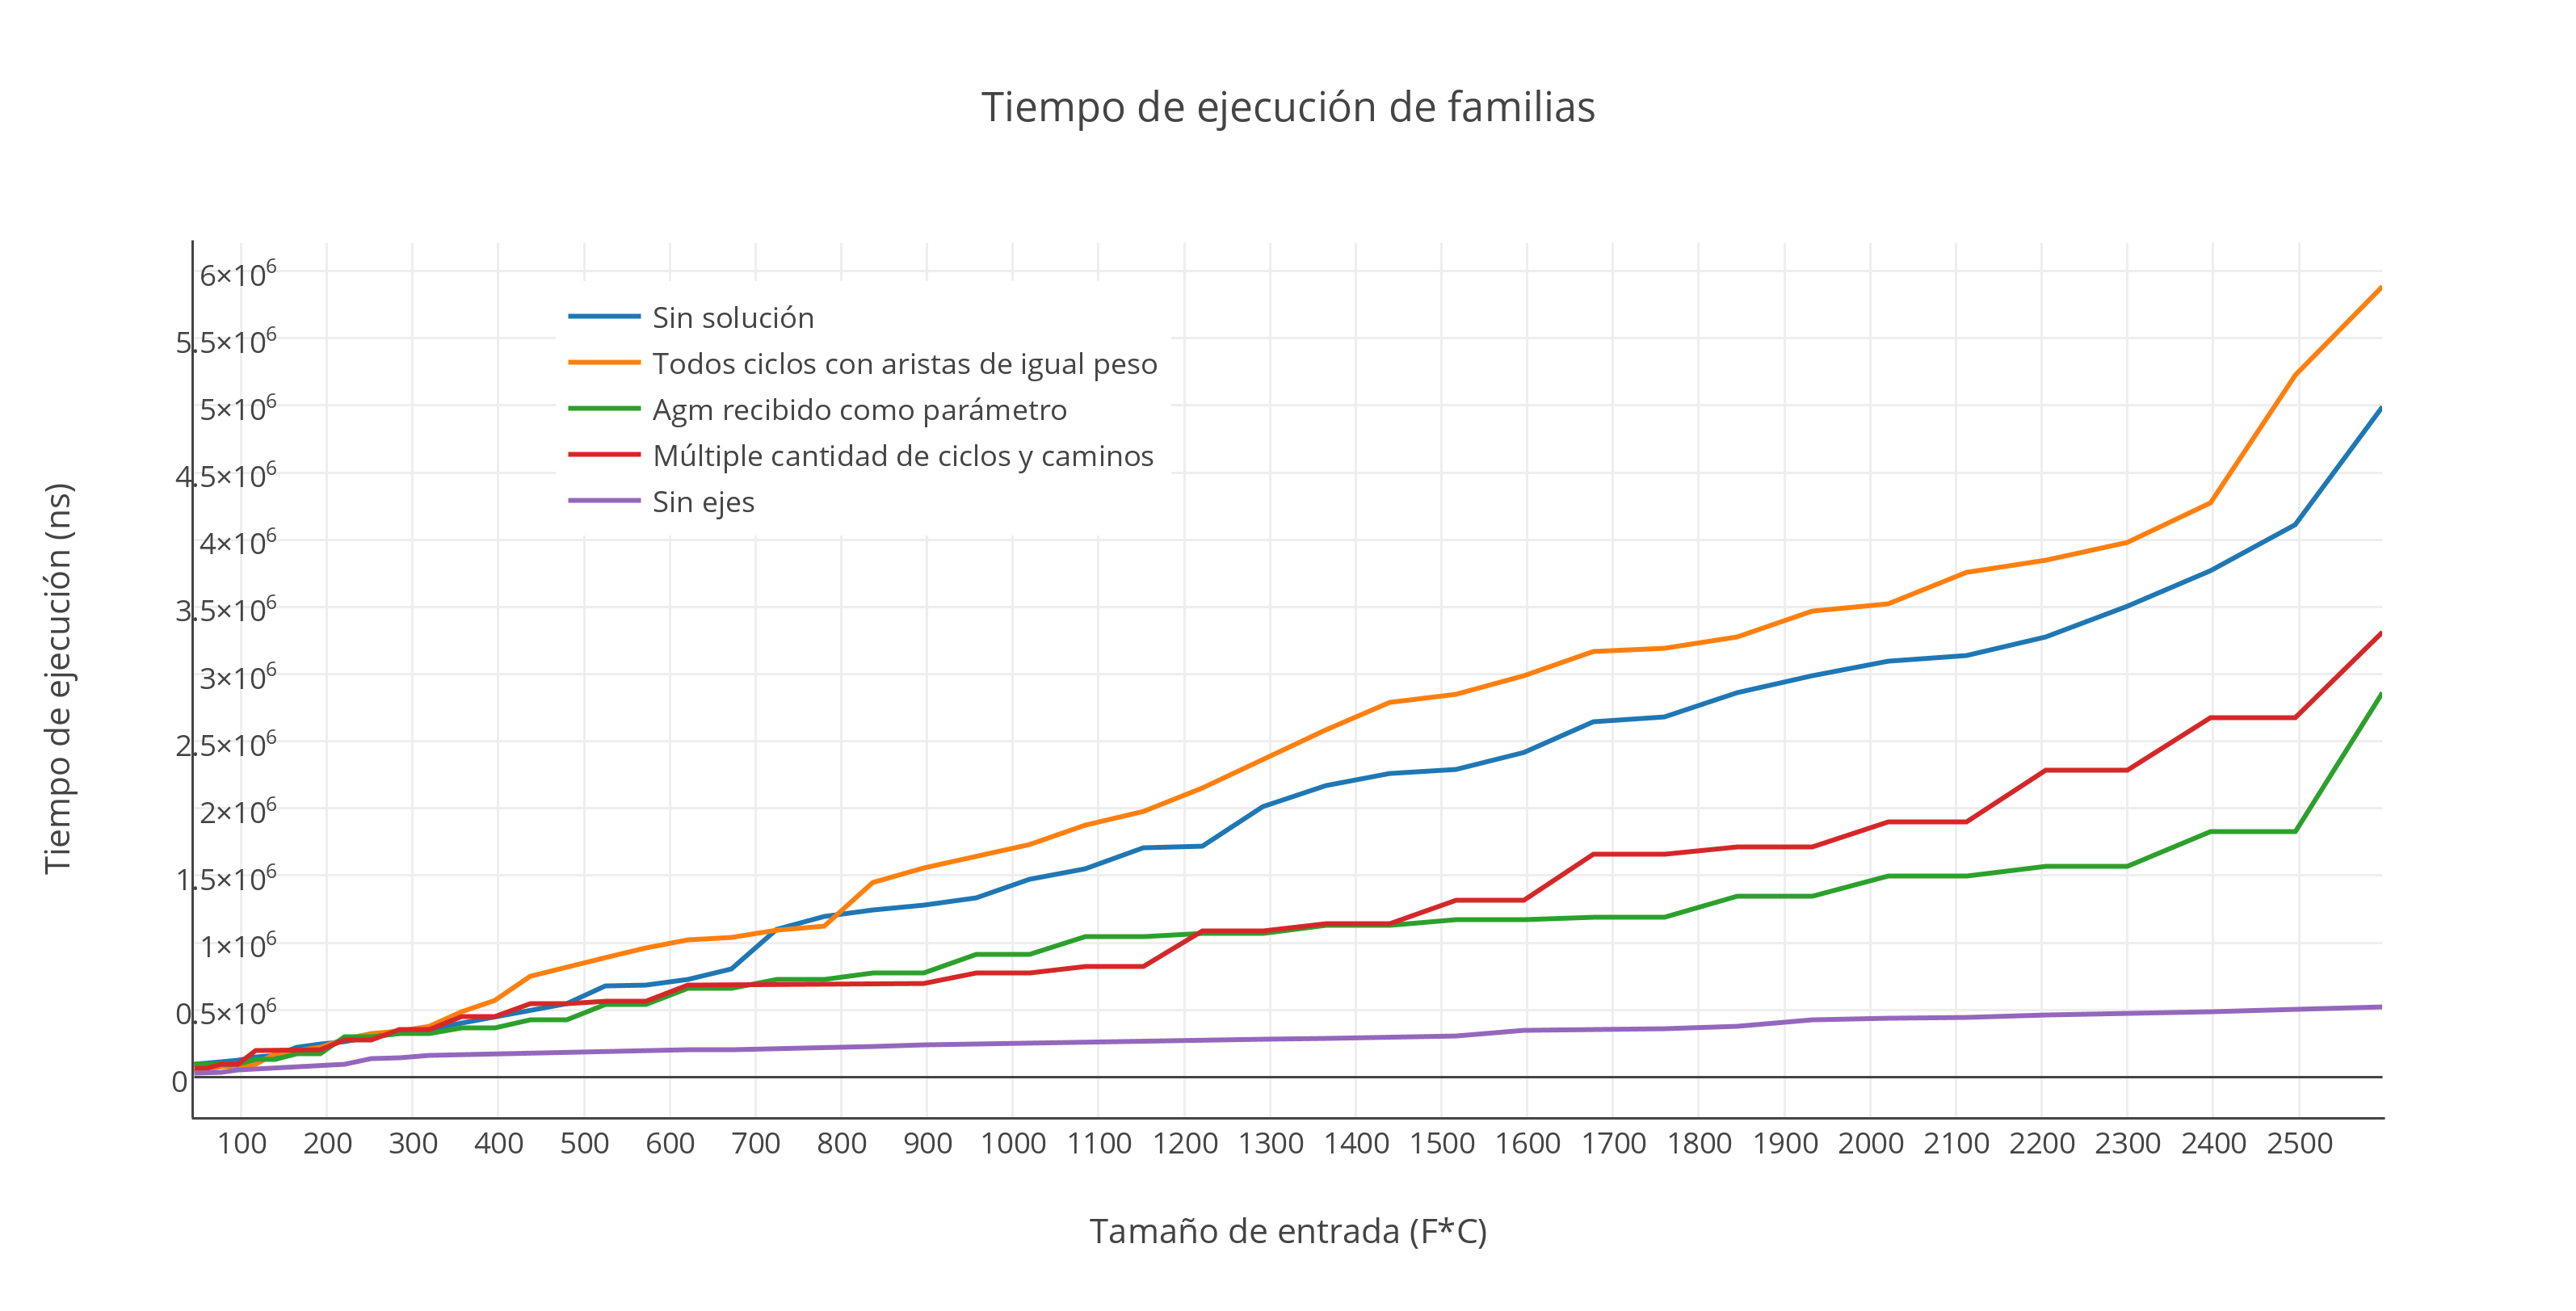
\includegraphics[scale=0.65]{./EJ2/comparativo.png}
 {$Gr$\'a$fico$ \ 2.1 - $Comparativo$}
  \end{center}
  \vspace*{0.3cm}
  
Se puede observar en el gr\'afico, cuatro funciones las cuales representan el tiempo de ejecuci\'on de las familias de casos:\\
\begin{itemize}
\item El grafo recibido como parametro es el AGM
\item No hay arbol posible que conecte a todas las componentes conexas
\item Existe un arbol de peso 0
\item El grafo recibido como parametro presenta multiples ciclos con aristas de disversos pesos
\end{itemize}

Como se observa en el gr\'afico la funci\'on representativa de la flia n\'umero 1, presenta una mejor performance en relaci\'on a las otras. Esto se debe a que nuestro algoritmo va chequeando los pesos de las aristas y observa que no se presenta ning\'un tipo de ciclo con posibilidad de bifuraci\'on de ramas del arbol, sino que hay un \'unico camino recorre dicho camino sumando los pesos y finaliza su ejecuci\'on.

Luego de chequear dichas instancias, pudimos llegar a la conclusi\'on que la familia de casos que presenta una mejor performance para nuestro algoritmo
es en el cual \textbf{el grafo que se obtiene de transformar el laberinto recibido como par\'ametro ya es el Arbol Generador M\'inimo}

Un grafo representativo de lo dicho ser\'ia el siguiente:

\vspace*{0.3cm} \vspace*{0.3cm}
  \begin{center}
 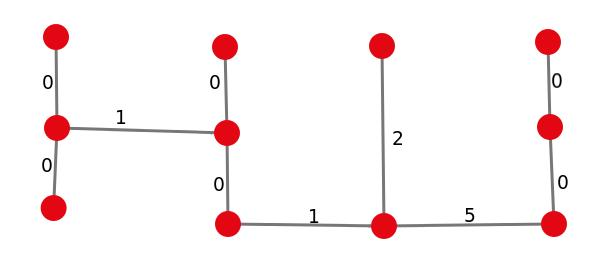
\includegraphics[scale=0.5]{./EJ2/ej2grafocompleto.jpeg}
 \\{$Grafo$ \ 2.1 - $Mejor$ $Caso$}
  \end{center}
  \vspace*{0.3cm}
  
Para llegar a dicha conclusi\'on trabajamos con 50 instancias.\\

Para una mayor observaci\'on desarrollamos el siguiente gr\'afico con las instancias:\\

\vspace*{0.3cm} \vspace*{0.3cm}
  \begin{center}
 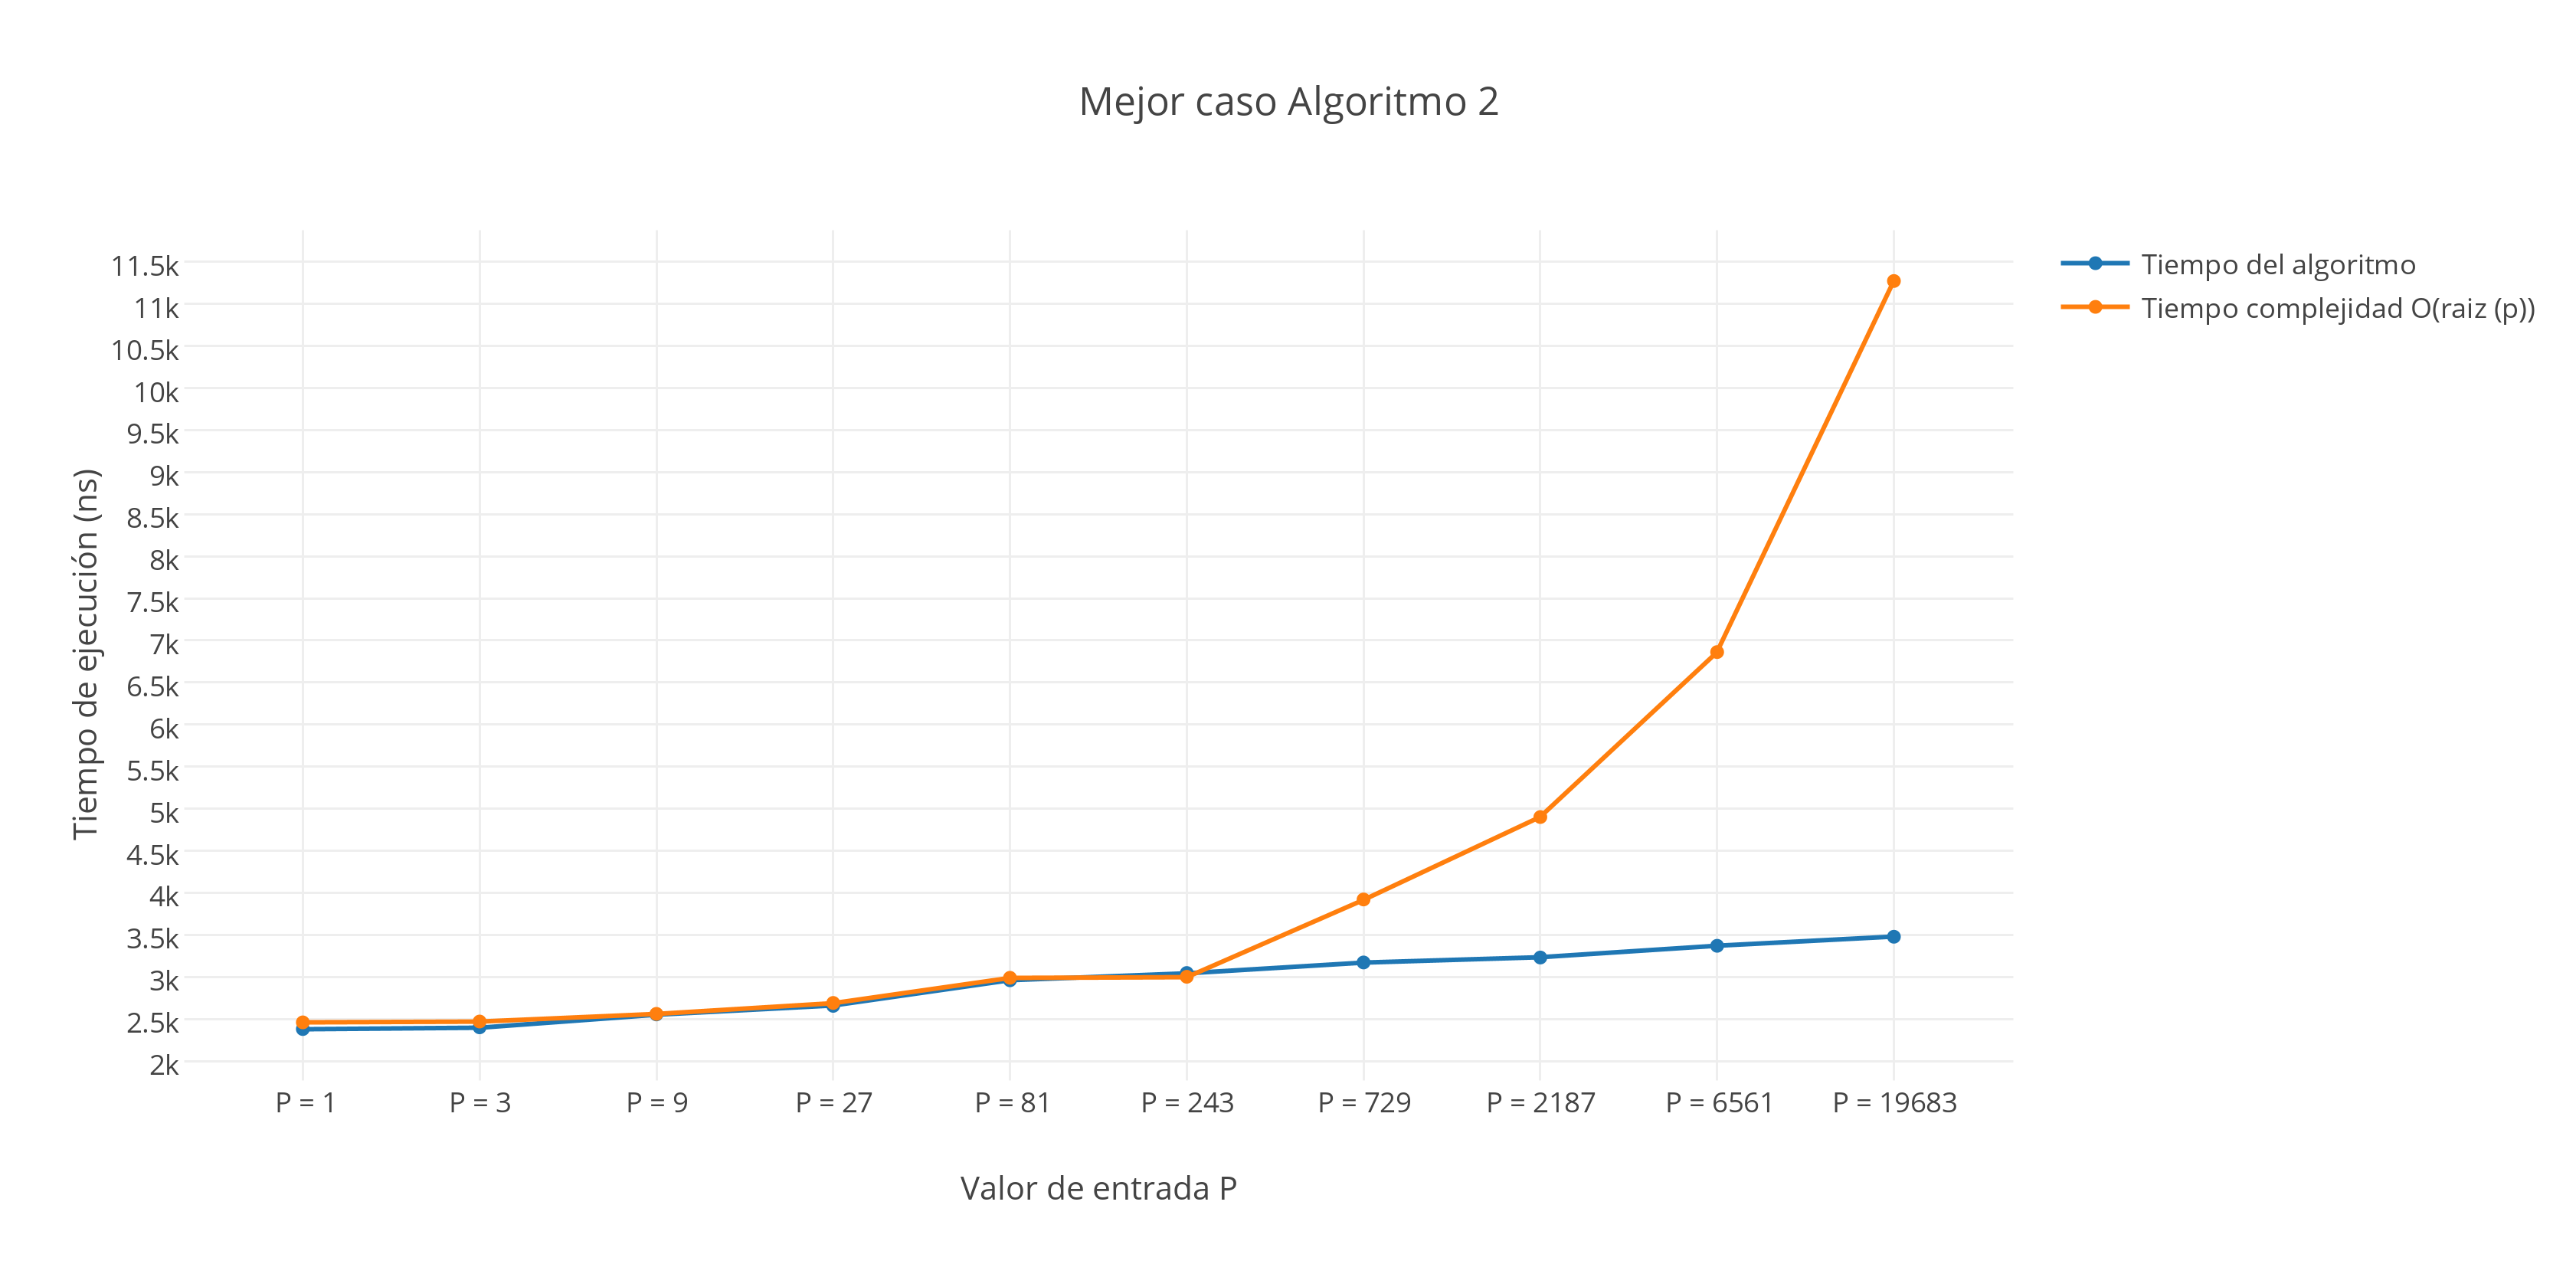
\includegraphics[scale=0.65]{./EJ2/mejorcaso.png}
 {$Gr$\'a$fico$ \ 2.1 - $Mejor Caso$}
  \end{center}
  \vspace*{0.3cm}
  
Como es posible observar en el gr\'afico, la funci\'on resultante de la cota teorica crece mucho m\'as r\'apido que la de nuestro algoritmo la cual queda considerablemente por debajo .

Luego, dividiendo por la complejidad teorica de nuestro algoritmo llegamos a:\\

\vspace*{0.3cm} \vspace*{0.3cm}
  \begin{center}
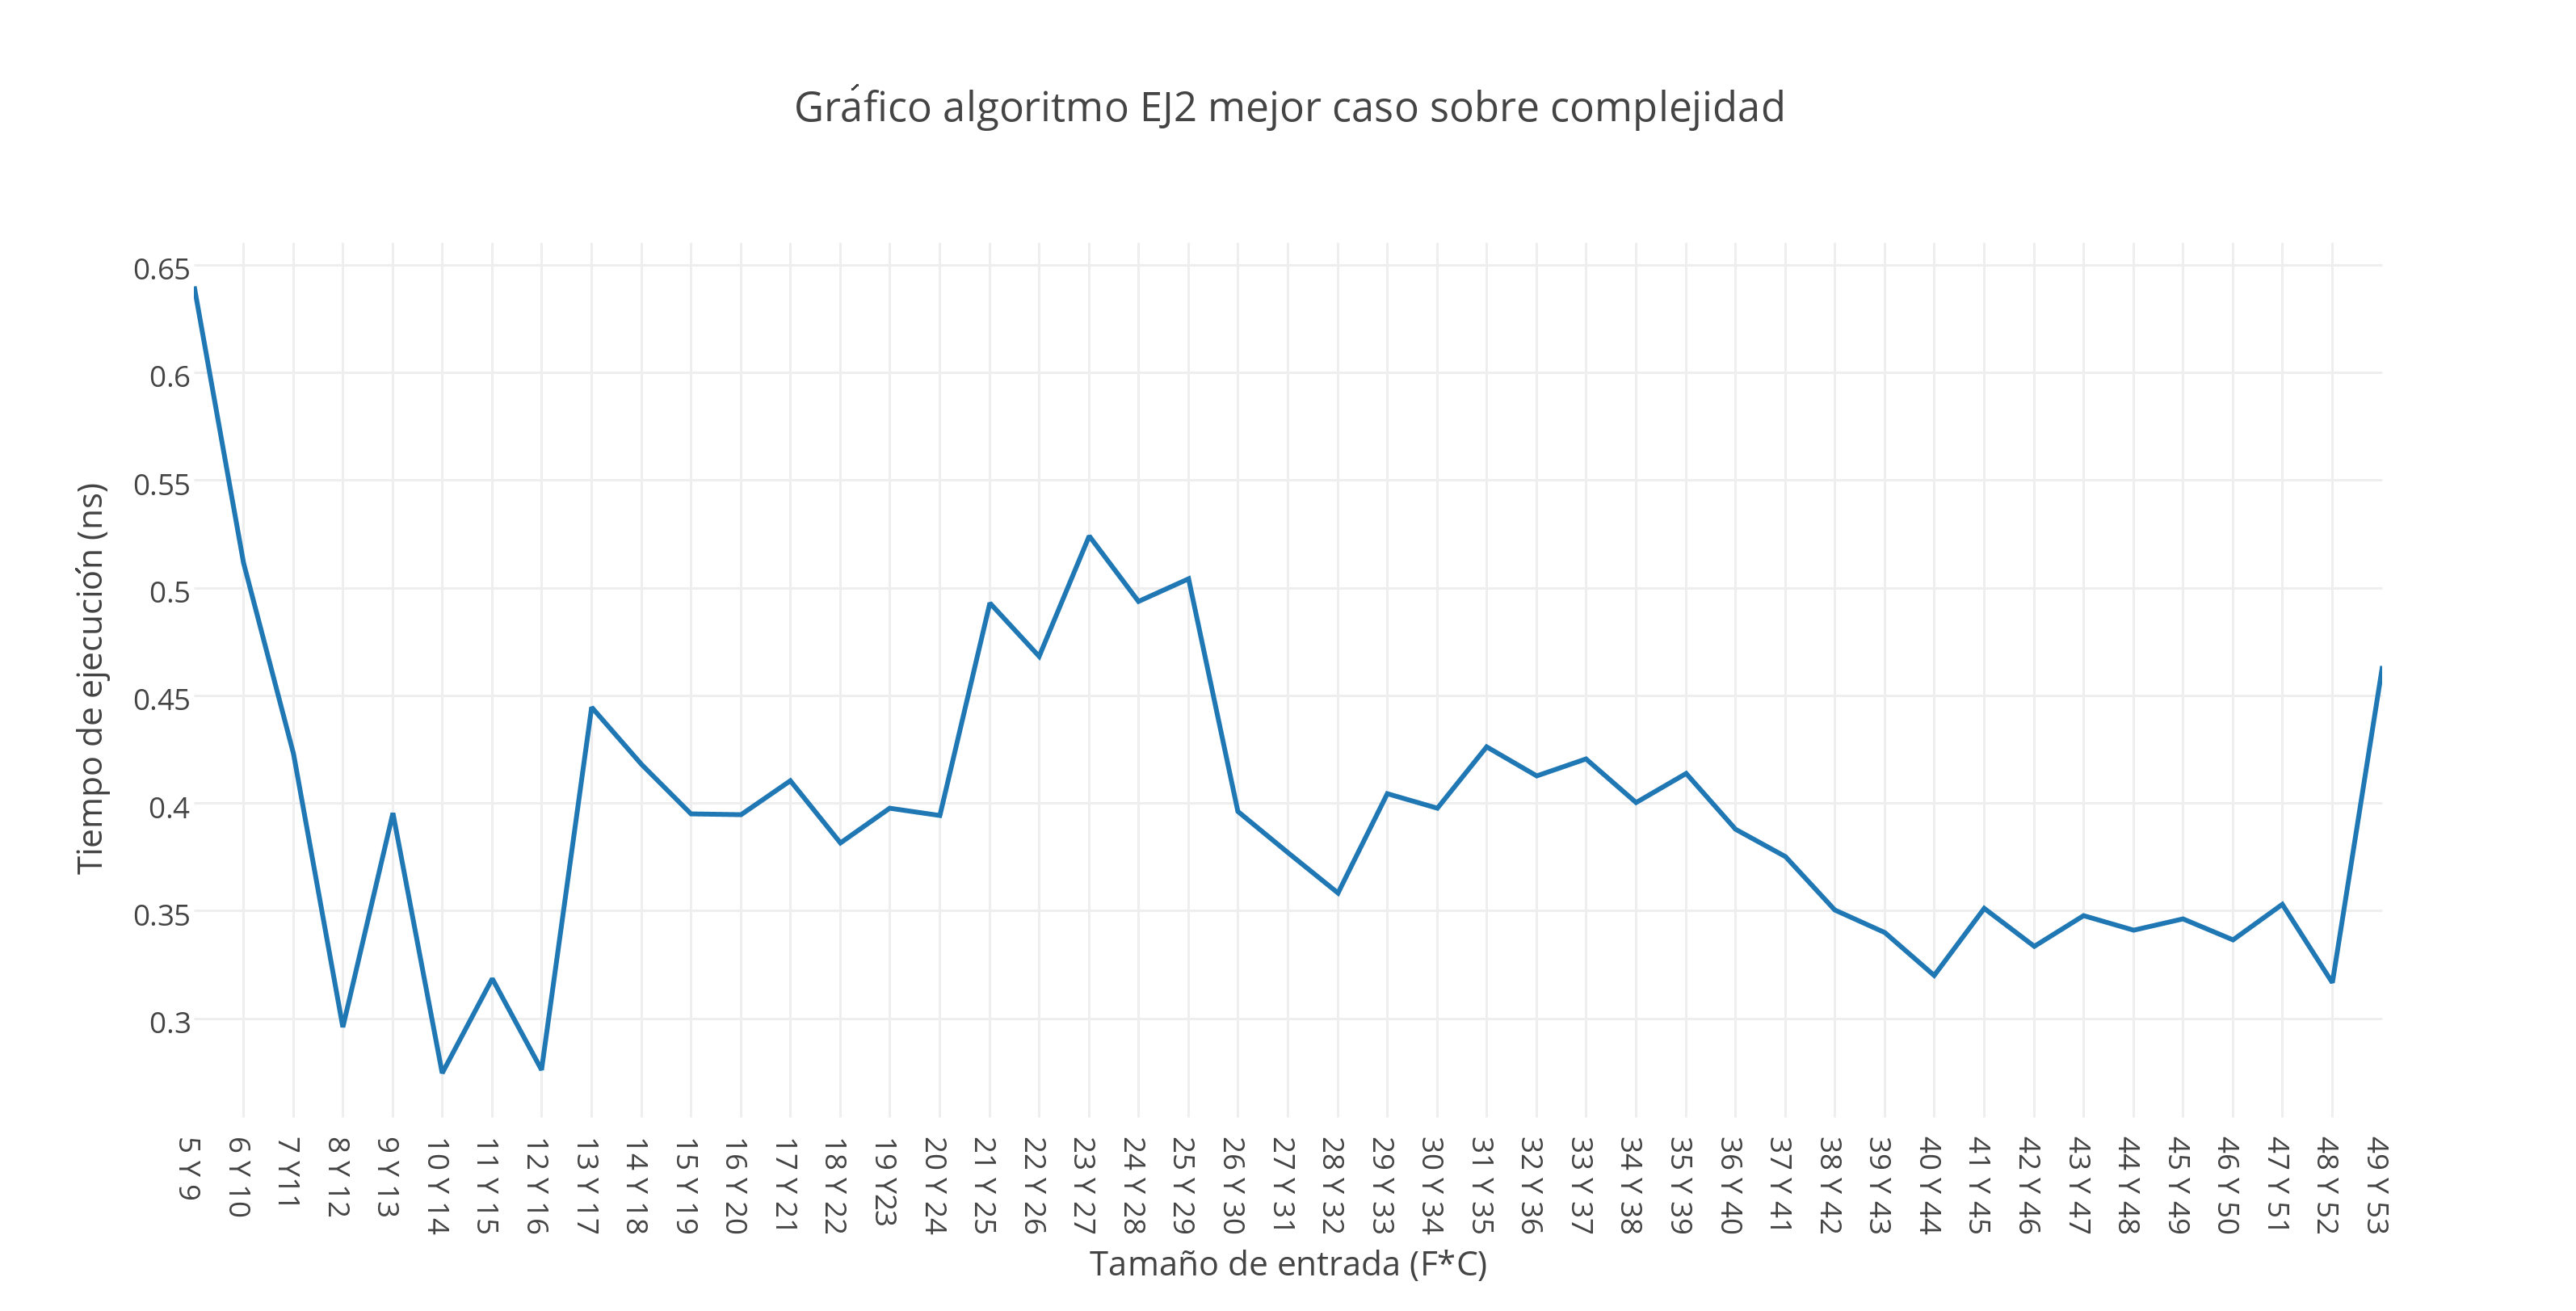
\includegraphics[scale=0.65]{./EJ2/mejorcaso1.png}
{$Gr$\'a$fico$ \ 2.2 - $Mejor Caso / Complejidad$ $O(F*C* log(F*C))$}
  \end{center}
  \vspace*{0.3cm}

Para realizar esta experimentaci\'on nos parecio prudente, realizar un promedio con el mismo input de aproximadamente 20 corridas
tanto para la complejidad como para nuestro algoritmo y una vez calculado dicho promedio de ambas cosas realizamos la divisi\'on para
obtener resultados m\'as relevantes.\\ 

Se puede observar en el gr\'afico 2.2, como luego de realizar la divisi\'on por la complejidad se ve que la funci\'on resultante tiene picos en los cuales llega a un m\'aximo igual a 0.65 y cuando el valor de entrada aumenta la funci\'on se asintotiza en 0.5. Por lo tanto, podemos concluir que para el mejor caso nuestro algoritmo se encuentra considerablemente por debajo de la cota teorica $O(F*C* log(F*C))$.\\

Luego, verificando el peor caso, llegamos a la conclusi\'on que la familia de casos en el que resulta menos beneficioso trabajar con nuestro algoritmo ser\'a cuando el grafo que se obtiene de transformar el laberinto de entrada es aquel que presenta un ciclo por cada habitaci\'on posible, dandonos el siguiente grafo una vez transformado:\\


\vspace*{0.3cm} \vspace*{0.3cm}
  \begin{center}
 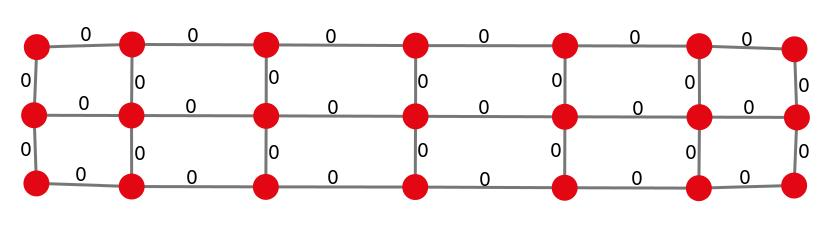
\includegraphics[scale=0.5]{./EJ2/ej2grafosinpared.jpeg}
 \\{$Grafo$ \ 2.2 - $Peor$ $Caso$}
  \end{center}
  \vspace*{0.3cm}
  
Realizando experimentos con un total de 50 instancias, desarrollamos dos gr\'aficos los cuales mostraremos a continuaci\'on: \\

\vspace*{0.3cm} \vspace*{0.3cm}
  \begin{center}
 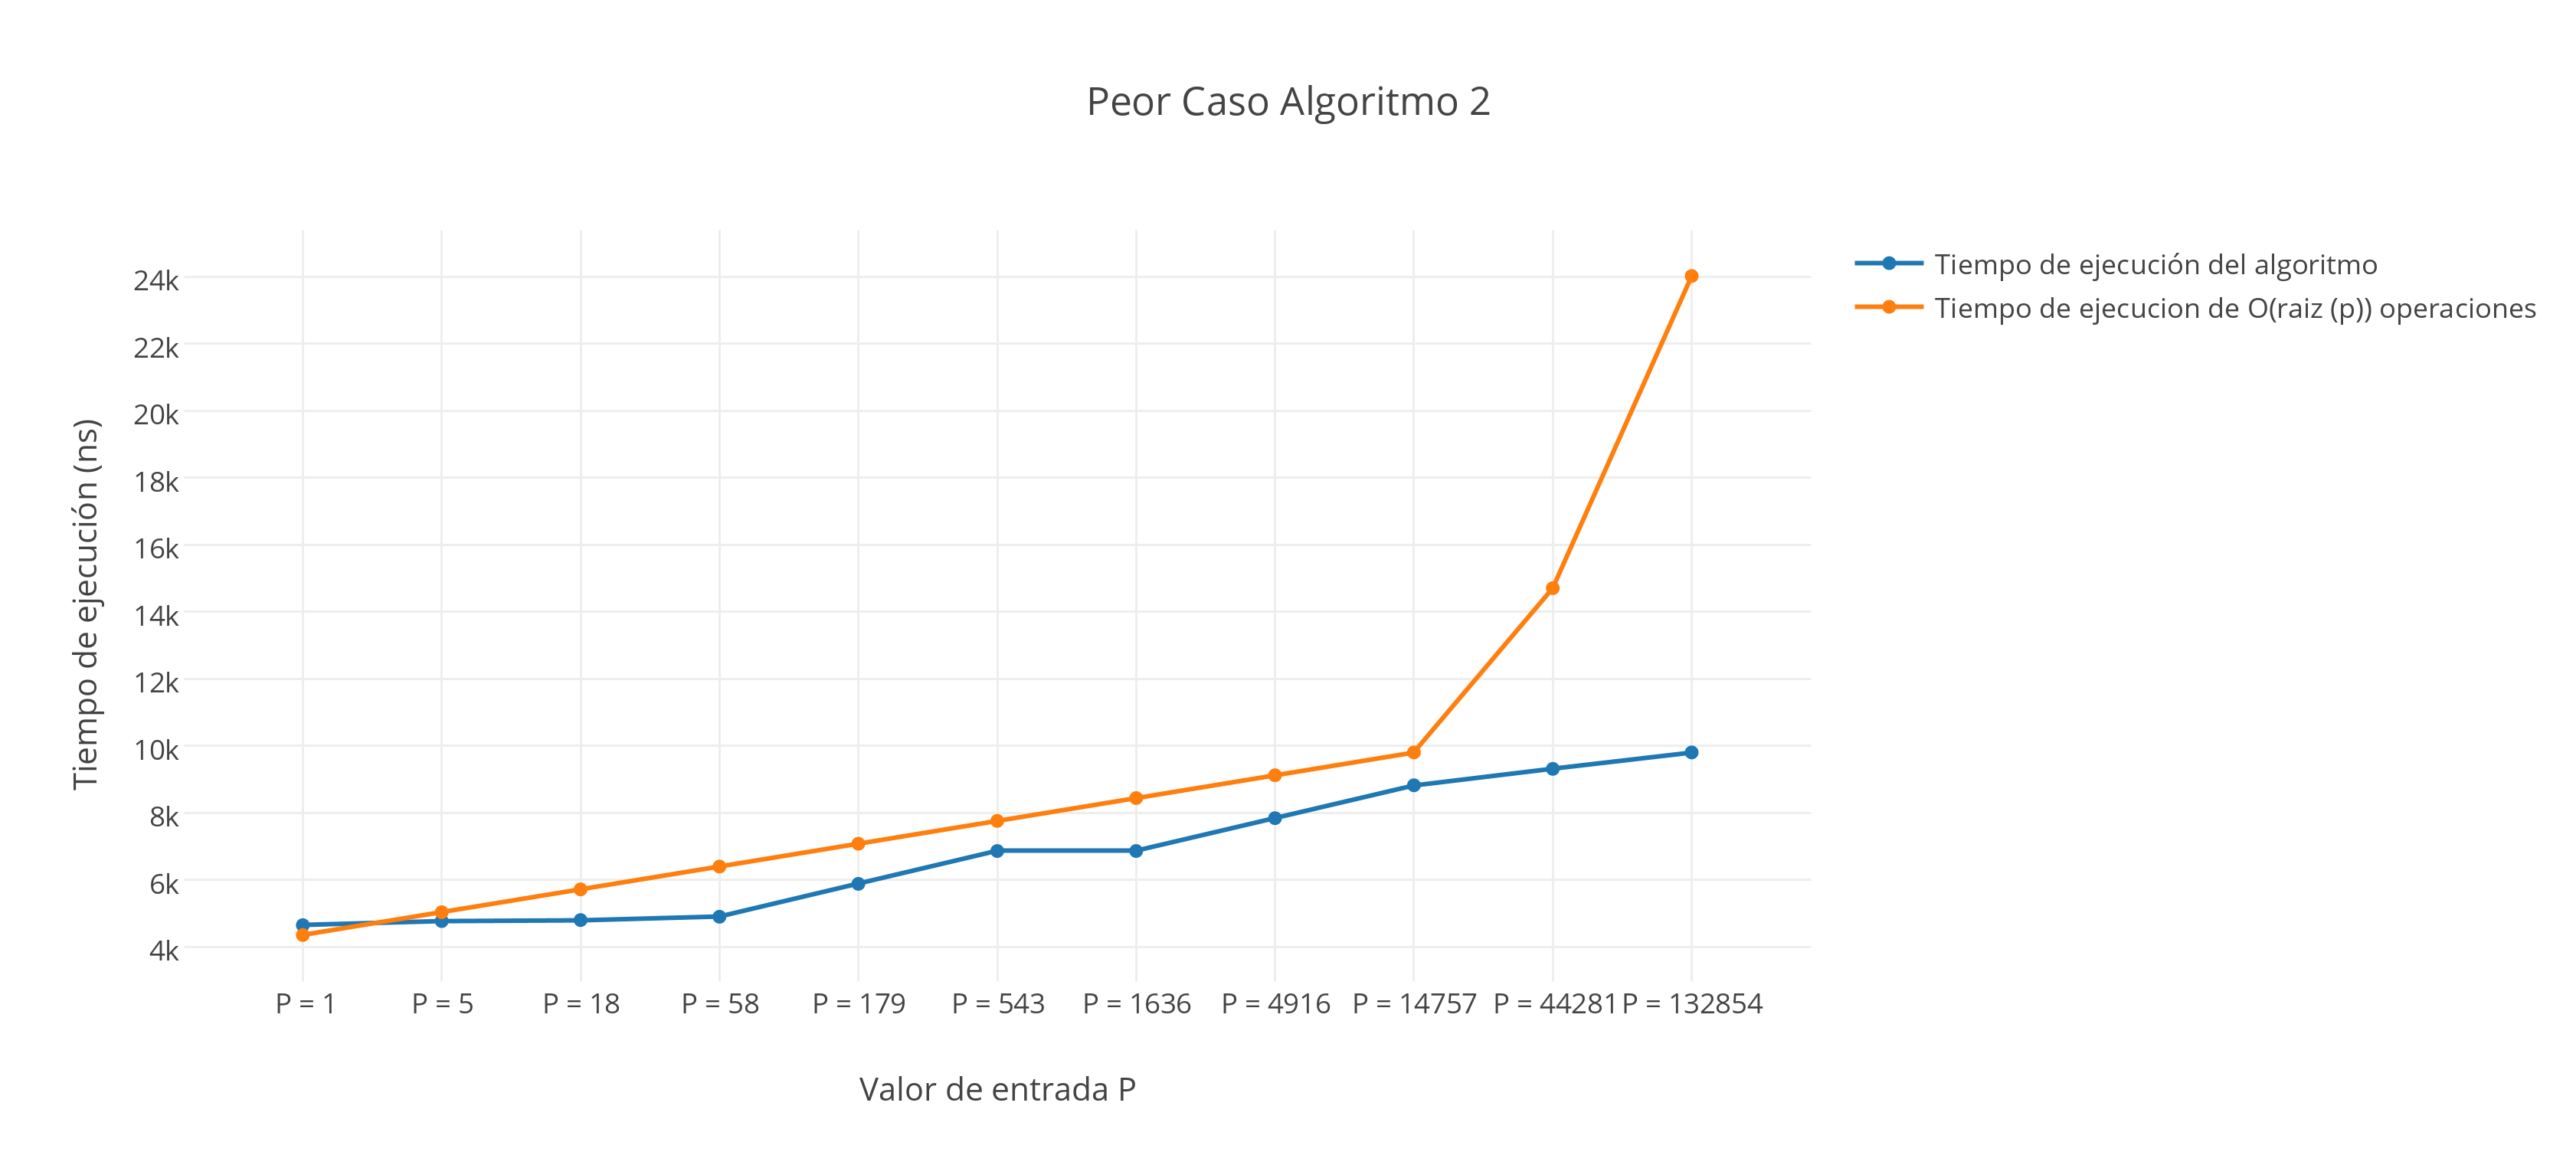
\includegraphics[scale=0.65]{./EJ2/peorcaso.png}
 {$Gr$\'a$fico$ \ 2.3 - $Peor Caso$}
  \end{center}
  \vspace*{0.3cm}


Dividiendo por la complejidad propuesta llegamos a:\\

\vspace*{0.3cm} \vspace*{0.3cm}
  \begin{center}
 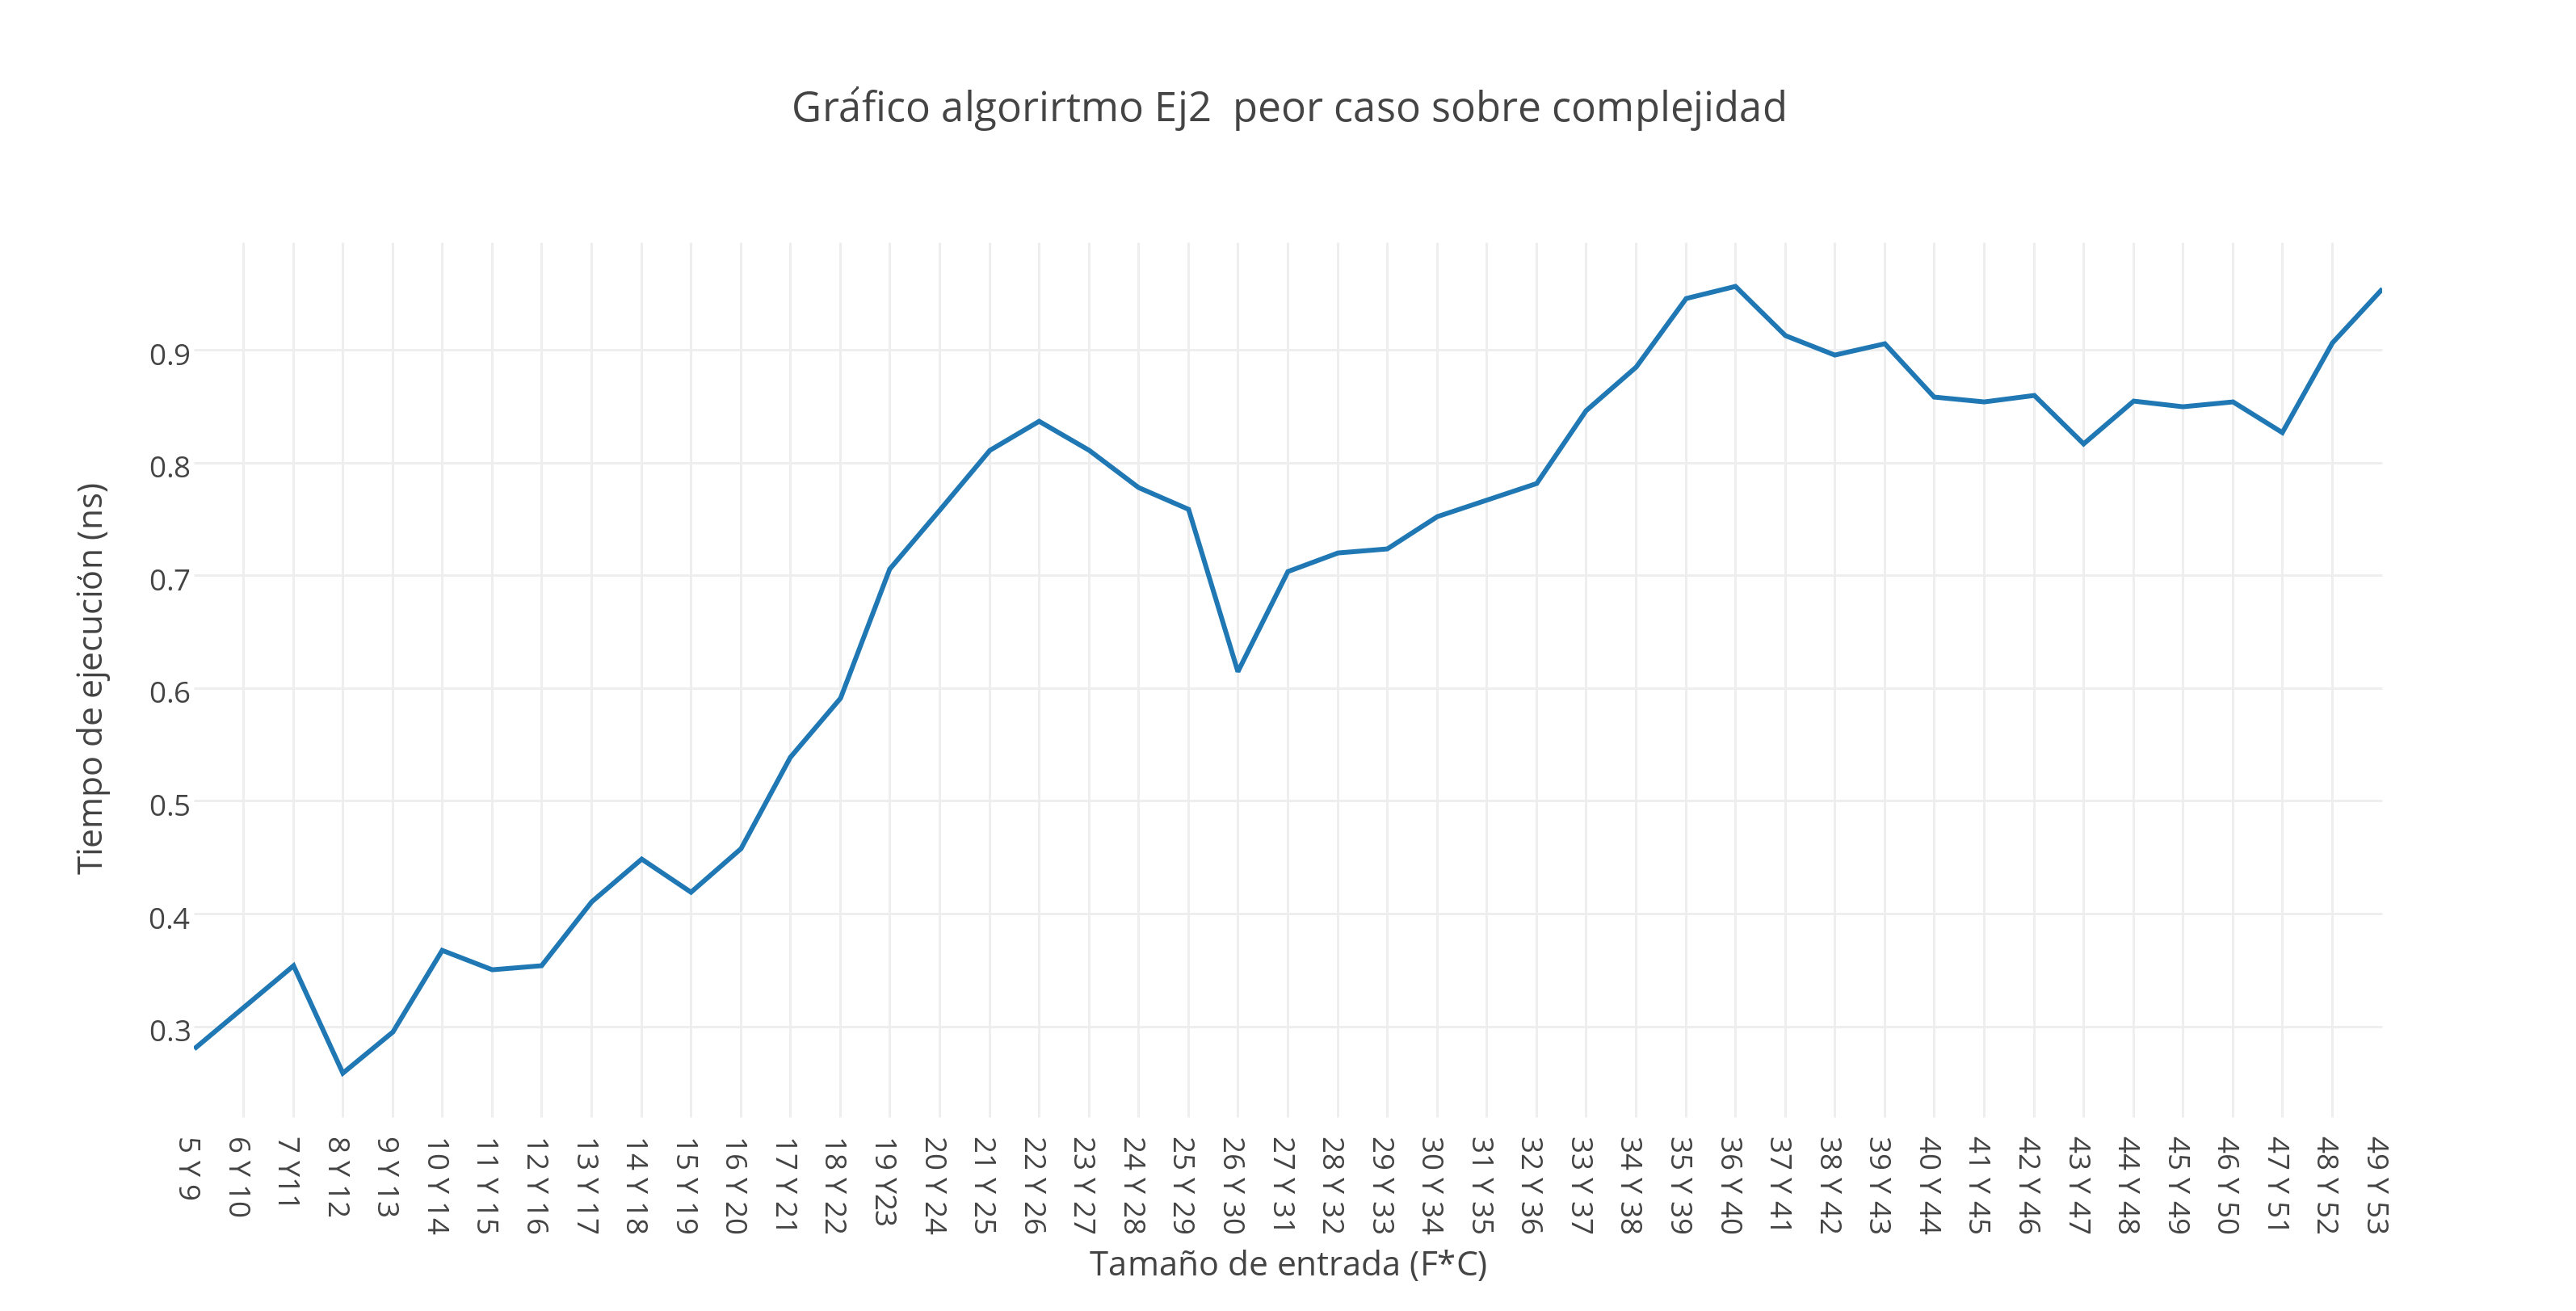
\includegraphics[scale=0.65]{./EJ2/peorcaso1.png}
 {$Gr$\'a$fico$ \ 2.4 - $Peor Caso / Complejidad$ $O(F*C* log(F*C))$}
  \end{center}
  \vspace*{0.3cm}

Para realizar esta experimentaci\'on nos parecio acorde, realizar un promedio con el mismo input de aproximadamente 20 corridas
tanto para la complejidad como para nuestro algoritmo y una vez calculado dicho promedio de ambas cosas realizamos la divisi\'on para
obtener resultados m\'as relevantes.\\ 

Como se puede observar en el gr\'afico 2.3, la funci\'on resultante de nuestro algoritmo es considerablemente mejor que la de la cota teorica  y presenta un tiempo similar al de la funci\'on resultante de la cota.
Luego, en el gr\'afico 2.4 se ve como la función resultante esta asintotizada por 1.\\

Por \'ultimo, mostraremos un gr\'afico comparativo entre el mejor y peor caso contra la complejidad que se solicito:\\

\vspace*{0.3cm} \vspace*{0.3cm}
  \begin{center}
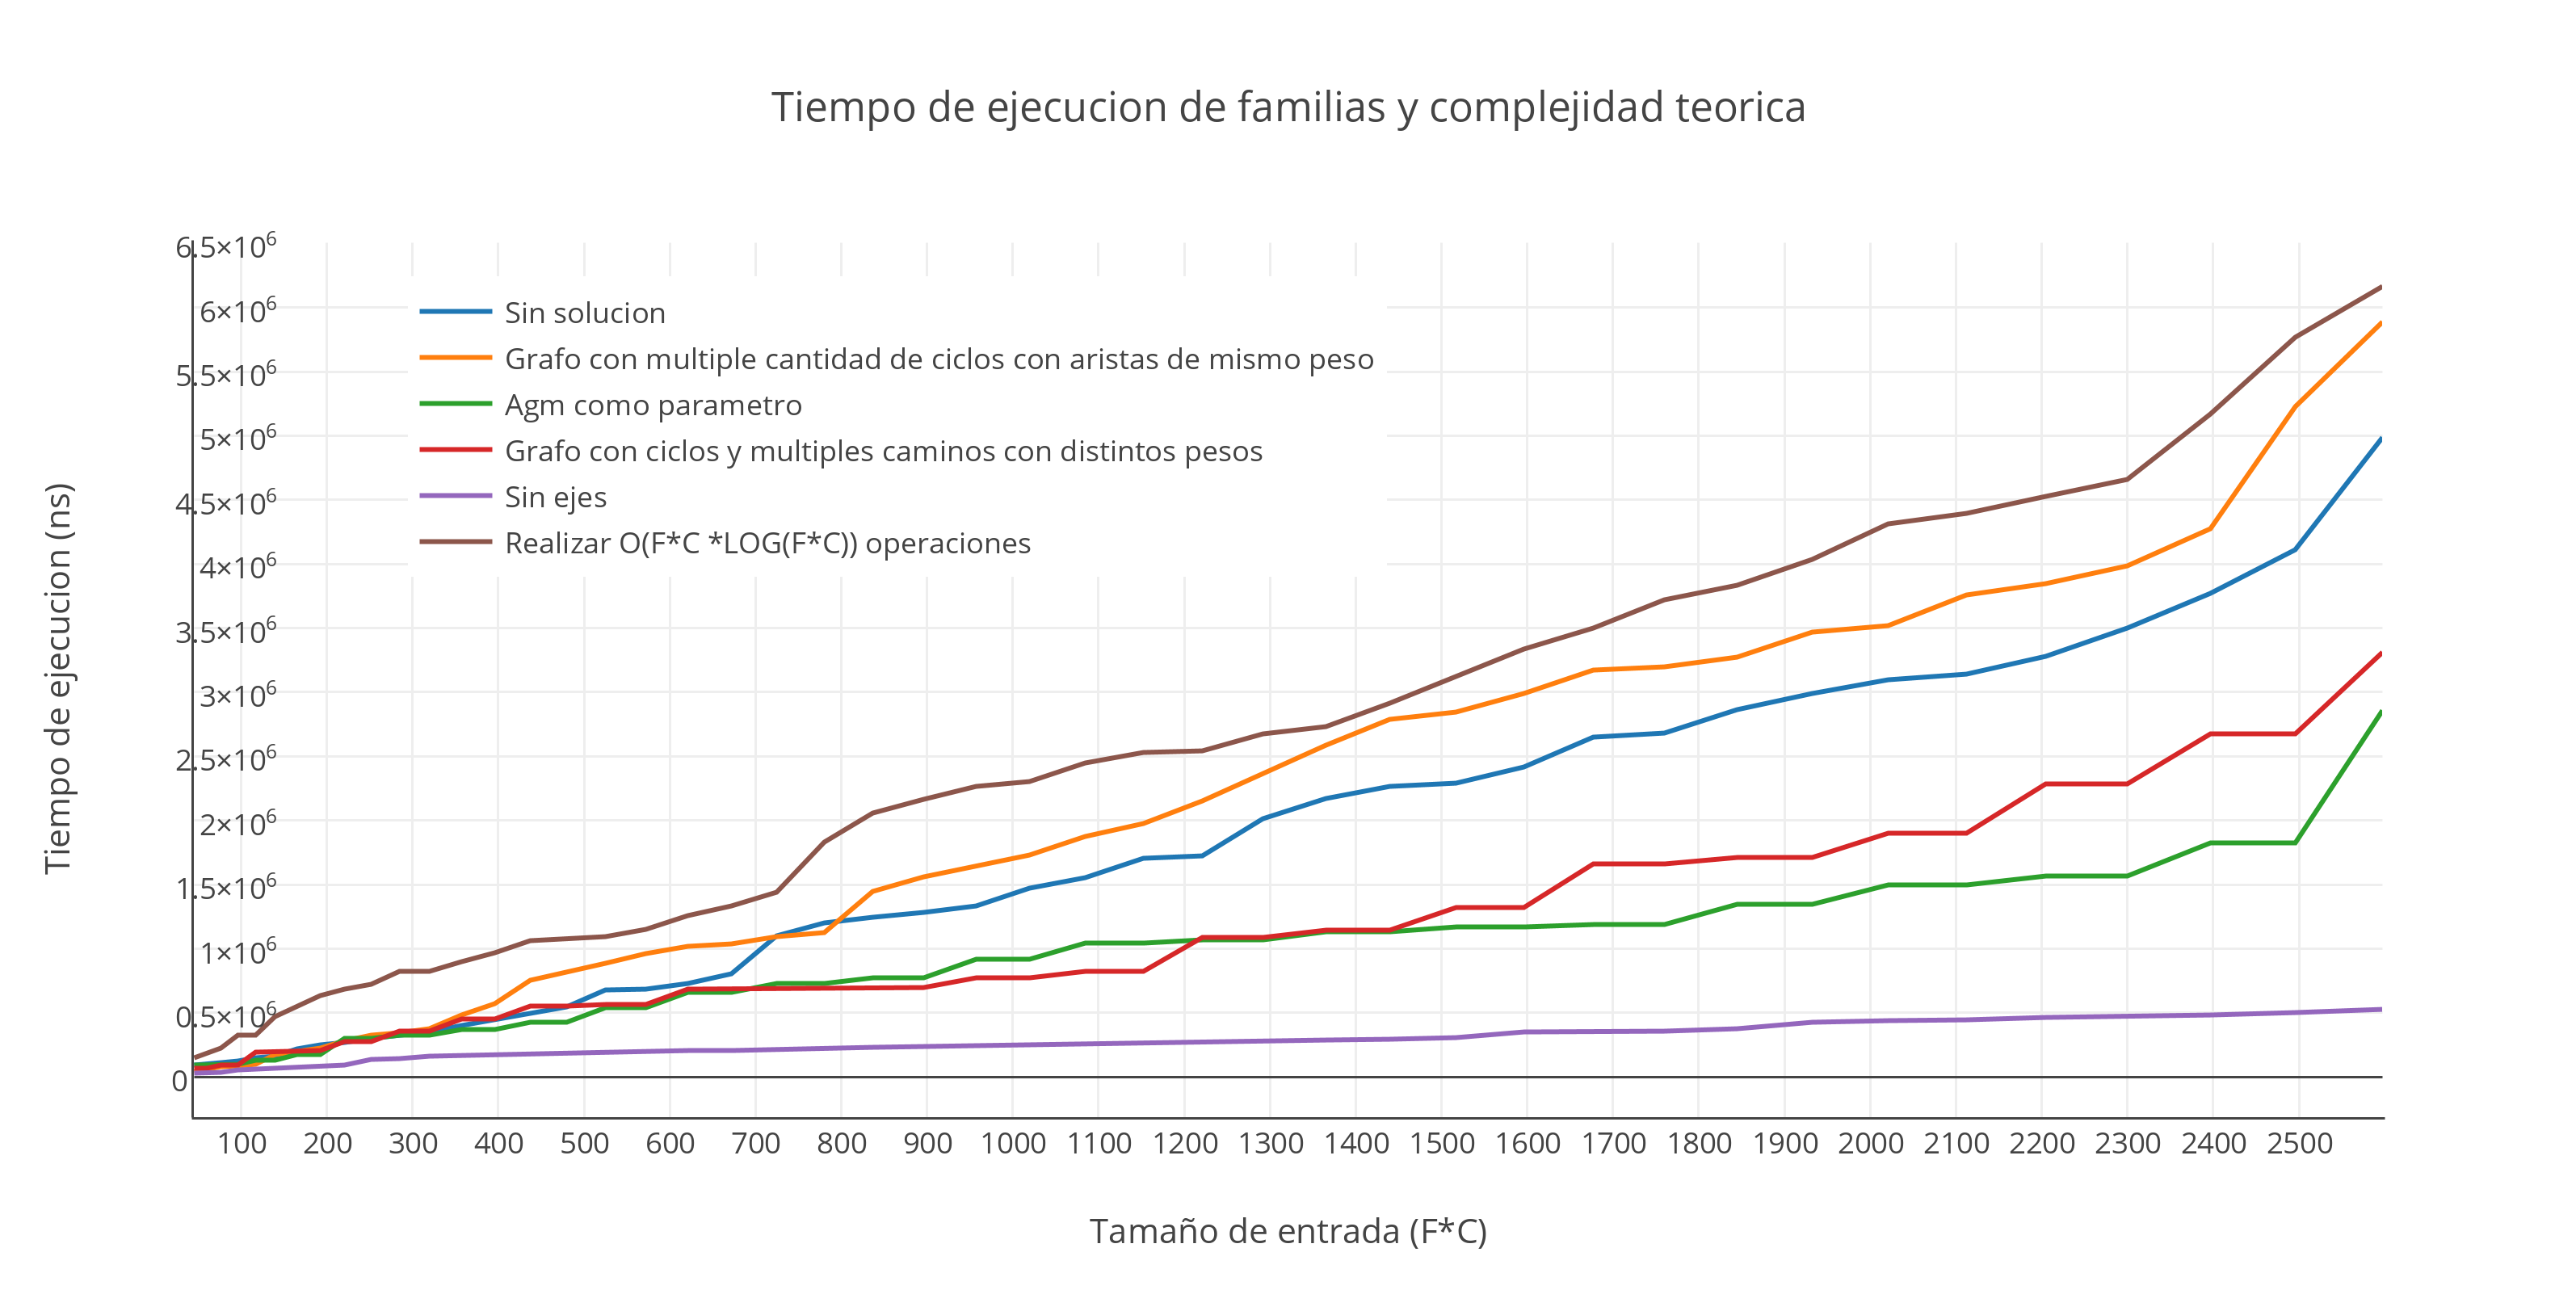
\includegraphics[scale=0.65]{./EJ2/comparativo1.png}
 {$Gr$\'a$fico$ \ 2.5 - $Comparativo$}
  \end{center}
  \vspace*{0.3cm}
  
Luego de dichos experimentos y casos probados, se puede concluir que a pesar de tener ciclos en todas las salas y donde dichos ciclos presenten aristas con pesos iguales lo que generara al algoritmo la posibilidad de crear varias ramas posibles de soluci\'on nos mantenemos dentro de la complejidad propuesta como hab\'iamos mostrado en nuestro desarrollo de la complejidad.\\
